\documentclass[a4paper,9pt,twocolumn,twoside,]{pinp}

%% Some pieces required from the pandoc template
\providecommand{\tightlist}{%
  \setlength{\itemsep}{0pt}\setlength{\parskip}{0pt}}

% Use the lineno option to display guide line numbers if required.
% Note that the use of elements such as single-column equations
% may affect the guide line number alignment.

\usepackage[T1]{fontenc}
\usepackage[utf8]{inputenc}

% pinp change: the geometry package layout settings need to be set here, not in pinp.cls
\geometry{layoutsize={0.95588\paperwidth,0.98864\paperheight},%
  layouthoffset=0.02206\paperwidth, layoutvoffset=0.00568\paperheight}

\definecolor{pinpblue}{HTML}{185FAF}  % imagecolorpicker on blue for new R logo
\definecolor{pnasbluetext}{RGB}{101,0,0} %



\title{Executive Summary Report}

\author[]{R10-08}


\setcounter{secnumdepth}{0}

% Please give the surname of the lead author for the running footer
\leadauthor{R10-08}

% Keywords are not mandatory, but authors are strongly encouraged to provide them. If provided, please include two to five keywords, separated by the pipe symbol, e.g:
 

\begin{abstract}
This report documents the process of how a regression model was selected
to predict the quality of red wine. First, 2 models were created using a
backwards stepwise approach and an AIC forward search. The backwards
model was selected and used to predict the quality of the wines using
the predictor values. The model was able to only predict ``normal''
quality wine (e.g.~5-6), due to the unbalanced nature of the dataset.
Further testing of selection methods, as regression tasks could be
considered for future study.
\end{abstract}

\dates{This version was compiled on \today} 

% initially we use doi so keep for backwards compatibility
% new name is doi_footer
\doifooter{\url{https://github.sydney.edu.au/kvoo2843/R10-08.git}}

\pinpfootercontents{Executive Summary Report - Wine Quality}

\begin{document}

% Optional adjustment to line up main text (after abstract) of first page with line numbers, when using both lineno and twocolumn options.
% You should only change this length when you've finalised the article contents.
\verticaladjustment{-2pt}

\maketitle
\thispagestyle{firststyle}
\ifthenelse{\boolean{shortarticle}}{\ifthenelse{\boolean{singlecolumn}}{\abscontentformatted}{\abscontent}}{}

% If your first paragraph (i.e. with the \dropcap) contains a list environment (quote, quotation, theorem, definition, enumerate, itemize...), the line after the list may have some extra indentation. If this is the case, add \parshape=0 to the end of the list environment.


\hypertarget{introduction}{%
\subsection{Introduction}\label{introduction}}

Using the dataset provided, we tried to create a suitable model that
determines the predictive power of the input variables. In our case, our
goal is to create a model that can be used to predict the quality of red
wine, based on the predictor variables selected, based on both a forward
and backwards stepwise variable selection process, and then choosing the
more suitable model, preferably the one with fewer variables. We will
then discuss the limitations and potential improvements to our model.

\hypertarget{dataset-description}{%
\subsection{Dataset Description}\label{dataset-description}}

This dataset is from the UCI Machine Learning Repository and contains
variables relating to the makeup of Portuguese ``Vinho Verde'' wines.
White wine and red wine is divided into two separate datasets. We chose
to only build a model on the red wine dataset, due to the specifications
asking for only one dataset to be analysed. There are a total of 1597
observations in this red wine dataset. This dataset in its current form
was originally intended to model wine preferences via machine learning.
A thing to note is that both datasets were stated to be unbalanced
(e.g.~there were many more ``normal'' quality wines than there were
great or bad ones).

Variables consist of both input and output variables. Input variables
include:

\begin{itemize}
\tightlist
\item
  \textbf{Fixed Acidity}: Acidity that naturally occurs in the grapes.
\item
  \textbf{Volitile Acidity}: Acidity produced from bacteria. High
  volatile acidity is known to be a sign of spoilage.
\item
  \textbf{Citric Acid}: Both added and naturally occurring. Most of it
  is fermented away in fermentation.
\item
  \textbf{Residual Sugar}: Natural sugars from grapes that did not
  ferment in the winemaking process.
\item
  \textbf{Chlorides}: Measurement of salt content
\item
  \textbf{Free Sulfur Dioxide}: Portion free in the wine
\item
  \textbf{Total Sulfur Dioxide}: Portion bonded to other chemicals in
  the wine
\item
  \textbf{Density}: Mass per volume
\item
  \textbf{PH}: Measurement of the wine's acidity
\item
  \textbf{Sulphates}: Additive from the winemaking process to allow
  freshness
\item
  \textbf{Alcohol}: Measurement of the overall alcohol proportion in the
  sample \newline(Winemaker's Academy, 2013)
\end{itemize}

The output variable is a quality rating out of 10. This is a discrete
set between 1 and 10 inclusive. Most quality scores were around 5 or 6
out of 10, with an interquartile range of 1, as shown in fig 1. A total
of 82\% of all observations received these scores. The top quality score
was 8, with the bottom quality score 3, providing a range of 5. But
there were much fewer observations the further away from Q1 and Q3 the
quality was. This can be seen in figure 1.

\begin{figure}

{\centering 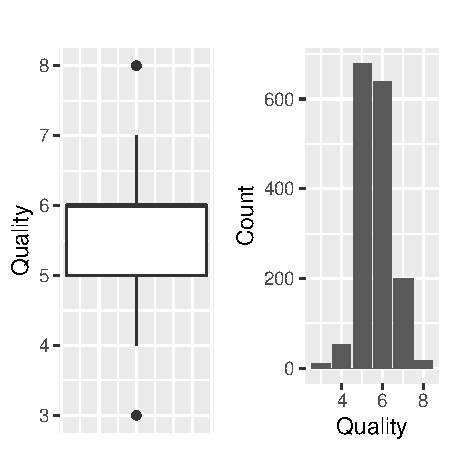
\includegraphics{Executive-Summary_files/figure-latex/figex-1} 

}

\caption{Boxplot and Histogram of Quality scores}\label{fig:figex}
\end{figure}

\hypertarget{analysis}{%
\subsection{Analysis}\label{analysis}}

We initially began work on our model selection by creating two different
models using 2 different approaches. The first model created was a
`Stepwise Backward' model, where we started with an initial full model
and reduced the size of the model by dropping variables that were
insignificant at the 5\% level of significance. We dropped the variables
in sequence, based on the largest p-values.

We eventually encountered a variable \emph{residual sugar}, that had a
p-value of around \textbf{0.13}. We decided to also drop the variable,
as although it is significant at the 5\% level of significance, it would
become insignificant at the 1\% level of significance. We then created
another Forward model using AIC, with R. Once we had our 2 models, we
then compared to see which of the 2 would be the more suitable model. We
noticed that the \(R^2\) values were almost identical, and the adjusted
\(R^2\) values were the same between the 2 models
\hyperref[table-1]{(see Table 1)}, and so we selected the model with the
least amount of variables out of the 2 as our model. That being the
Stepwise Backward model \hyperref[table-1]{(see Table 1 (1))}.

\hypertarget{the-final-model-can-be-defined-as}{%
\subsubsection{The final model can be defined
as:}\label{the-final-model-can-be-defined-as}}

\begin{equation}
  \begin{aligned}
  quality = \beta_{0} + \beta_{1}{x_1} + \beta_{2}{x_2} + \beta_{3}{x_3} + ... + \beta_{7}{x_7} + \beta_{8}{x_8} + \epsilon_i
       \label{eqn:model}
  \end{aligned}
\end{equation}

\begin{itemize}
\tightlist
\item
  \(x_1\) = volatile acidity
\item
  \(x_2\) = density
\item
  \(x_3\) = sulphates
\item
  \(x_4\) = chlorides
\item
  \(x_5\) = total sulfur dioxide
\item
  \(x_6\) = citric acid
\item
  \(x_7\) = free sulfur dioxide
\item
  \(x_8\) = alcohol
\end{itemize}

Once we had our model, we began to check the regression assumptions for
our selected model. \pagebreak

\hypertarget{assumption-checking}{%
\subsubsection{Assumption checking}\label{assumption-checking}}

\begin{itemize}
\tightlist
\item
  \textbf{Linearity}: Upon observing the residual vs fitted values plot,
  the graph showed elements of linearity as there was no obvious pattern
  shown in the graph, such as a parabolic shape. As such, the normal
  assumption is not violated, and it doesn't appear that we have
  misspecified the model.
\item
  \textbf{Independence}: Based on the nature of the dataset, we assumed
  that each sampling of wine does not affect the other wine samples. We
  also assumed the wines were chosen at random. That would mean all
  errors are independent of each other. Furthermore, the dataset we are
  working with does not deal with time-series data, reducing the
  likelihood of the independence assumption being violated. As such, the
  independence assumption is at least approximately satisfied.\\
\item
  \textbf{Homoskedasticity}: Based on the scatter plot, the residuals
  for each fitted value appears mostly equal in the spread, apart for
  some outliers. So, the constant error variance assumption is met.
\item
  \textbf{Normality}: In the QQ plot, it is very obvious that the points
  are reasonably close to the diagonal line. The bottom left endpoints
  are not quite on the line but are not severe enough to influence the
  results. As such, the normality assumption is at least approximately
  satisfied.
\end{itemize}

\begin{figure}

{\centering 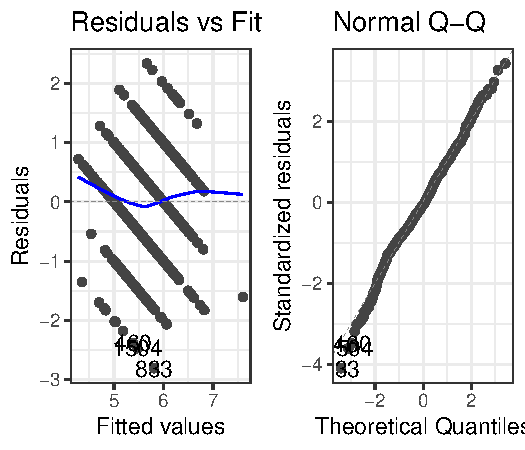
\includegraphics{Executive-Summary_files/figure-latex/unnamed-chunk-3-1} 

}

\caption{Checking linear assumptions for the backwards stepwise model.}\label{fig:unnamed-chunk-3}
\end{figure}

\hypertarget{results}{%
\subsection{Results}\label{results}}

Looking at the \(R^2\) value from the summary output
\hyperref[table-1]{(see Table 1)}, 28\% (see discussion for details) of
the variability of the wine quality is explained by the regression on
the 8 predictor variables in our model.

Using the final model, we can estimate the average quality of wine or
the quality of a single sample of wine with specific properties
(predictor variables). By using a confidence interval to estimate the
average quality and, a prediction interval for predicting a single
sample of wine. A thing to note is that the full model is not
particularly good at making predictions on exceptionally
``good''(e.g.~8+) or ``bad'' (e.g.~\textless4) wines, as the dataset is
very unbalanced (e.g.~most values were around 5 or 6).

Below is a quick demonstration of a prediction interval prediction using
the first entry from the dataset.

\begin{ShadedResult}
\begin{verbatim}
#  Rows: 1
#  Columns: 8
#  $ volatile_acidity     <dbl> 0.7
#  $ citric_acid          <dbl> 0
#  $ chlorides            <dbl> 0.076
#  $ free_sulfur_dioxide  <dbl> 11
#  $ total_sulfur_dioxide <dbl> 34
#  $ density              <dbl> 0.9978
#  $ alcohol              <dbl> 94
#  $ quality              <dbl> 5
\end{verbatim}
\end{ShadedResult}
\begin{ShadedResult}
\begin{verbatim}
#         fit      lwr      upr
#  1 5.176034 3.829332 6.522736
\end{verbatim}
\end{ShadedResult}

The predicted quality was about 5.18, which was roughly the same as the
actual quality value in the dataset which was 5.

\hypertarget{model-performance}{%
\subsubsection{Model Performance}\label{model-performance}}

The `root mean square error' value was found to be 0.68
\hyperref[figure-1]{(see Figure 1 in Appendix)}. When accounting for
outliers, the mean absolute error was calculated at 0.54, which is a
stronger measurement for this dataset due to the large cluster of
quality scores around 5 and 6. In contrast, the null model returned a
root mean square error of 0.81 and a mean absolute error of 0.68, which
was lower than the values for the full model. For the full model, 10
fold cross-validation also returned the same values for MAE and RMSE.

\hypertarget{discussion-conclusion}{%
\subsection{Discussion \& Conclusion}\label{discussion-conclusion}}

When we first plotted our residuals vs fitted values and QQ-plot graphs,
we then noticed the unorthodox shape of the residual vs fitted graph. We
then realised that it was due to the dependent variable, quality, being
discrete values. We made an attempt to log the dependent variable in an
attempt to improve the shape of the graph, but there were no noticeable
changes to the model and decided to leave the values discrete.

A thing to note is that the \(R^2\) values were low, at approximately
28\%. As mentioned before, this was maybe due to the dataset being
unbalanced.

In an attempt to improve the results, the model was reduced further by
dropping the variable \emph{alcohol}. Although significant even at the
1\% level of significance with a p-value of about 0.025, it was by far
the largest p-value amongst the other values. However, this did not
improve the overall \(R^2\) value, and the changes that occurred were
negligible. As such, we decided to stick with our final model that is
shown \hyperref[eqn:model]{above}.

To try to improve the equal variance assumption, logging the dependent
variable was tested. This was also attempted with the independent
variables. Despite this, there was no improvement in the overall
variance of the model. The weakness of the assumptions may have affected
the \(R^2\) value of the model.

In retrospect, an improvement that could have been made was to perform
formal tests to see if the coefficient for each variable we were going
to drop were significant when creating our model. By first defining a
model with the relevant parameters, and then forming formal hypothesis
and assumptions, do the relevant assumption checks, find the test
statistic, and p-values, conclude whether or not to drop the
variable(s). This was not done, due to time and severe labour
constraints.

Another improvement would have been using a classification model to
predict quality as a discrete factor. The use of linear regression
returned predicted quality values on a continuous scale, despite all
recorded qualities being integers from 1 to 10. The use of a
classification model would have also taken into account the major
influence that the observations with qualities of 5 or 6 play in the
regression model.

\pagebreak

\hypertarget{references}{%
\subsection{References}\label{references}}

\begin{itemize}
\tightlist
\item
  Understanding Wine Acidity. (2018, June 25). Retrieved from
  \url{http://winemakersacademy.com/understanding-wine-acidity/}.
\item
  P. Cortez, A. Cerdeira, F. Almeida, T. Matos and J. Reis. Modeling
  wine preferences by data mining from physicochemical properties. In
  Decision Support Systems, Elsevier, 47(4):547-553, 2009.
\item
  Broman KW (2015) R/qtlcharts: interactive graphics for quantitative
  trait locus mapping. Genetics 199:359-361
\item
  Hadley Wickham, Romain François, Lionel Henry and Kirill Müller
  (2019). dplyr: A Grammar of Data Manipulation. R package version
  0.8.3. \url{https://CRAN.R-project.org/package=dplyr}
\item
  H. Wickham. ggplot2: Elegant Graphics for Data Analysis.
  Springer-Verlag New York, 2016.
\item
  Lüdecke D (2019). \emph{sjPlot: Data Visualization for Statistics in
  Social Science}. doi: 10.5281/zenodo.1308157 (URL:
  \url{http://doi.org/10.5281/zenodo.1308157}), R package version 2.7.2,
  \textless URL:
  \url{https://CRAN.R-project.org/package=sjPlot}\textgreater.
\item
  Yuan Tang, Masaaki Horikoshi, and Wenxuan Li. ``ggfortify: Unified
  Interface to Visualize Statistical Result of Popular R Packages.'' The
  R Journal 8.2 (2016): 478-489.
\item
  Hlavac, Marek (2018). stargazer: Well-Formatted Regression and Summary
  Statistics Tables. R package version 5.2.1.
  \url{https://CRAN.R-project.org/package=stargazer}
\end{itemize}

\hypertarget{appendix}{%
\subsection{Appendix}\label{appendix}}

\hypertarget{table-1}{%
\subsubsection{Table 1}\label{table-1}}

\begin{itemize}
\item
  \begin{enumerate}
  \def\labelenumi{(\arabic{enumi})}
  \tightlist
  \item
    = Stepwise Backward Model.
  \end{enumerate}
\item
  \begin{enumerate}
  \def\labelenumi{(\arabic{enumi})}
  \setcounter{enumi}{1}
  \tightlist
  \item
    = AIC Forward Model.
  \end{enumerate}
\end{itemize}

\begin{table}[!htbp] \centering 
  \caption{Regression Results} 
  \label{} 
\begin{tabular}{@{\extracolsep{5pt}}lcc} 
\\[-1.8ex]\hline 
\hline \\[-1.8ex] 
 & \multicolumn{2}{c}{\textit{Dependent variable:}} \\ 
\cline{2-3} 
\\[-1.8ex] & \multicolumn{2}{c}{quality} \\ 
\\[-1.8ex] & (1) & (2)\\ 
\hline \\[-1.8ex] 
 volatile\_acidity & $-$0.909$^{***}$ & $-$0.923$^{***}$ \\ 
  & (0.126) & (0.126) \\ 
  & & \\ 
 citric\_acid & 0.629$^{***}$ & 0.610$^{***}$ \\ 
  & (0.122) & (0.123) \\ 
  & & \\ 
 chlorides & $-$3.288$^{***}$ & $-$3.274$^{***}$ \\ 
  & (0.410) & (0.410) \\ 
  & & \\ 
 free\_sulfur\_dioxide & 0.005$^{***}$ & 0.005$^{***}$ \\ 
  & (0.001) & (0.001) \\ 
  & & \\ 
 total\_sulfur\_dioxide & $-$0.006$^{***}$ & $-$0.006$^{***}$ \\ 
  & (0.001) & (0.001) \\ 
  & & \\ 
 density & $-$86.012$^{***}$ & $-$87.214$^{***}$ \\ 
  & (10.337) & (10.365) \\ 
  & & \\ 
 sulphates & 1.246$^{***}$ & 1.252$^{***}$ \\ 
  & (0.116) & (0.116) \\ 
  & & \\ 
 alcohol & 0.000$^{**}$ & 0.000$^{**}$ \\ 
  & (0.000) & (0.000) \\ 
  & & \\ 
 residual\_sugar &  & 0.001 \\ 
  &  & (0.0004) \\ 
  & & \\ 
 Constant & 91.326$^{***}$ & 92.516$^{***}$ \\ 
  & (10.268) & (10.295) \\ 
  & & \\ 
\hline \\[-1.8ex] 
Observations & 1,597 & 1,597 \\ 
R$^{2}$ & 0.283 & 0.284 \\ 
Adjusted R$^{2}$ & 0.280 & 0.280 \\ 
Residual Std. Error & 0.686 (df = 1588) & 0.685 (df = 1587) \\ 
F Statistic & 78.409$^{***}$ (df = 8; 1588) & 69.999$^{***}$ (df = 9; 1587) \\ 
\hline 
\hline \\[-1.8ex] 
\textit{Note:}  & \multicolumn{2}{r}{$^{*}$p$<$0.1; $^{**}$p$<$0.05; $^{***}$p$<$0.01} \\ 
\end{tabular} 
\end{table}

\hypertarget{figure-1}{%
\subsubsection{Figure 1}\label{figure-1}}

Output of the 10-fold cross validation - using the caret package.

\begin{ShadedResult}
\begin{verbatim}
#  Linear Regression 
#  
#  1597 samples
#     8 predictor
#  
#  No pre-processing
#  Resampling: Cross-Validated (10 fold) 
#  Summary of sample sizes: 1438, 1436, 1436, 1437, 1437, 1438, ... 
#  Resampling results:
#  
#    RMSE       Rsquared   MAE      
#    0.6889542  0.2754941  0.5418699
#  
#  Tuning parameter 'intercept' was held constant at a value of TRUE
\end{verbatim}
\end{ShadedResult}

%\showmatmethods


\bibliography{pinp}
\bibliographystyle{jss}



\end{document}

